\chapter{Agenti}
\section{Introduzione}
Nell'Intelligenza artificiale si è passati da Classical AI verso la Distribuited
AI.
\begin{definizione}[\textbf{Intelligent Agent}]
    Si definisce \textbf{Intelligent Agent} come lo studio degli agenti che
    ricevono delle percezioni dall'ambiente ed effettuano delle azioni su di esso.
\end{definizione}
Possiamo definire l'intelligenza artificiale attraverso lo studio di agenti,
stiamo \textbf{Agentification of AI}.
\begin{definizione}[\textbf{Agentification AI}, \textbf{Classical AI}]
    Con il termine \textbf{Agentification AI} ci riferiamo a una situazione in
    cui un singolo agente risolve problemi adottando diverse tecniche e approcci.
\end{definizione}
\section{Agente}
Il termine \textbf{agente} viene definito in diversi modi da diversi autori,
vogliamo ora riportare alcune definizioni di agente:
\begin{definizione}[Russel e Norvig]
    Un \textbf{agente} è qualcosa che percepisce l'ambiente attraverso sensori e
    agisce su di esso attraverso attuatori.
\end{definizione}
\begin{esempio}[Esempio di agente]
    Un esempio sono gli agenti umani composti da sensori come occhi, orecchie e
    altri organi, mentre è composto da attuatori che sono mani, gambe, bocca e
    parti del corpo.

    Un ulteriore esempio possono avere agenti robotici composti dai rispettivi
    sensori e attuatori.
\end{esempio}

Di un agente possiamo definire la \textbf{funzione agente} che mappa la storia
delle percezioni in una azione, ovvero:
\begin{equation}
    f: P^* \rightarrow A
\end{equation}
dove $P^*$ è l'insieme delle parti delle sequenze di percezioni e $A$ è l'insieme
delle azioni. Questa funzione può essere rappresentata in diversi modi:
\begin{itemize}
    \item \textbf{Production system}
    \item \textbf{Reactive agents}
    \item \textbf{Real-time conditional planners}
    \item \textbf{Neural network}
    \item \textbf{Decision-theorem system}
\end{itemize}

\begin{figure}[!ht]
    \centering
    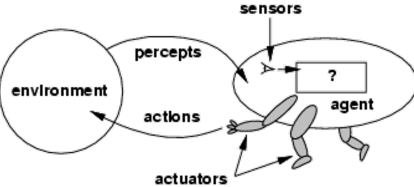
\includegraphics[width=0.5\textwidth]{./img/Agenti/AgenteEAmbiente.png}
    \caption{Schema di un agente}
    \label{fig:agenti}
\end{figure}

L'agente sarà anche formato dal \textbf{programma} dell'agente che viene
eseguito sulla sua \textbf{architettura} fisica per svolgere la funzione agente.
\begin{center}
    Agent = Program + Architecture
\end{center}
\begin{definizione} [\textbf{Distribuited AI}]
    La \textbf{Distribuited AI} consiste in un sistema di entità le quali possono
    risolvere un problema effettuando delle azioni e interagendo con l'ambiente,
    sia in collaborazione, sia in competizione.
\end{definizione}
A differenza della Classical AI in cui si ha un solo agente, nella Distribuited AI
si ha un sistema di agenti.
\begin{definizione} [\textbf{Sistema}]
    Un \textbf{sistema} è un gruppo di elementi che formano un insieme che
    collabora per raggiungere un obiettivo comune. Questo ci dice che un sistema
    è qualcosa in più di un singolo insieme di elementi, in quanto è presente un
    organizzazione tra le parti che lo compongono.
\end{definizione}
Prima abbiamo accennato a un sistema di entità che collaborano per risolvere un
problema, questo sistema può essere distribuito. Vogliamo ora capire cosa
può essere distribuito:
\begin{itemize}
    \item \textbf{Distribuited solving of problem}: la soluzione di un problema
          è distribuita, ovvero la soluzione del problema richiede capacità che
          appartengono a più entità.
    \item \textbf{Solving of distribuited problem}: distribuzione a livello di
          dominio del problema. In questo caso si può adottare una soluzione
          centralizzata. Un esempio di questa casistica è data dal coordinamento
          di robot in un magazzino.
    \item \textbf{Distribuited techniques for problem solving}: distribuzione a
          livello di tecniche da utilizzare per la risoluzione del problema.
\end{itemize}
\begin{esempio}[Distribuited solving of problem]
    Un esempio di problema non distribuito che viene risolto in modo distribuito
    è il riconoscimento del parlato. In questo caso si ha un sistema di agenti
    che collaborano per risolvere il problema. Sono presenti diversi livelli
    gerarchici, ogni livello si occupa di un particolare task.
\end{esempio}
\begin{esempio}[Solving of distribuited problem]
    Un esempio di problema distribuito che viene risolto in modo centralizzato è
    legato alla gestione di un magazzino. In questo caso si ha un sistema centrale
    che riceve le informazioni degli attuatori (robot) e comunica agli attuatori le
    azioni da svolgere. I vantaggi dell'approccio centralizzato sono la
    configurabilità e la predicibilità, quindi posso dimostrare proprietà. Posso
    predire malfunzionamenti degli agenti, quindi posso sovradimensionare la
    struttura per gestire i probabili malfunzionamenti. Si ha quindi una scalabilità,
    flessibilità e adattabilità limitata.

    Una soluzione alternativa è quella di convertire il sistema trasformando i
    muletti da attuatori ad agenti i quali comunicano col sistema centrale per
    effettuare i task. Passando quindi da un paradigma:
    \begin{center}
        muletto x porta al posto y un prodotto z
    \end{center},
    a uno del tipo:
    \begin{center}
        chi si offre di portare al posto y il prodotto z?
    \end{center}
    A questo punto i muletti risponderanno e il sistema selezionerà il migliore.
    Aumenta la complessità degli agenti perché devono gestire le richieste centrali
    e inoltre deve comunicare con gli altri agenti per non scontrarsi negli
    incroci. Quindi gli agenti devono avere una rappresentazione dell'ambiente,
    cosa che non avevano nella soluzione centralizzata, perché questo veniva
    gestito tutto dal server centrale.
\end{esempio}
\begin{esempio}[Distribuited techniques for problem solving]
    Un esempio sono i nemici di un videogioco che cooperano che sconfiggere il
    giocatore. Rappresento e gestisco i bot come agenti.
\end{esempio}

Nel passato per implementare la distribuited AI si avevano diversi metodi:
\begin{itemize}
    \item \textbf{Memoria distribuita}: struttura dati condivisa con problemi
          sull'accesso concorrente e con strategie di controllo degli agenti.
          Implementato con Linda che suggerisce un nuovo modo per gestire la
          concorrenza.
    \item \textbf{Processing autonomo} concorrente e il coordinamento tra gli
          agenti con scambio di messaggi. Implementato con modello ad Attori.
\end{itemize}
Attualmente, si utilizzano delle metodologie basate su middleware per sistemi
distribuiti ad esempio attraverso code o meccanismi di publish and subscribe
etc$\dots$ Degli esempi di tecnologie che implementano questi meccanismi sono
Redis e Kafka.

Gli approcci basati su sistemi di agenti presentano diverse criticità:
\begin{itemize}
    \item Il sistema viene modellato definendo l'ambiente, l'architettura e poi
          si ragiona sul singolo agente. Non per tutti i sistemi si può ragionare
          sul singolo agente. Spesso esistono azioni eseguite dagli agenti che
          vanno a influenzare l'ambiente.
    \item La modifica sull'ambiente può limitare la scelta delle azioni degli
          agenti quindi l'autonomia spesso non è buona e complica la gestione
          degli agenti.
\end{itemize}
\section{Architettura degli agenti}
Una prima classificazione degli agenti è quella di Genesereth la quale si basa
sul fatto che gli agenti possono essere classificati in base alle loro capacità
interne e alle risorse a loro disposizione. Questa prima classificazione
distingue gli agenti in:
\begin{itemize}
    \item \textbf{Tropistic}
    \item \textbf{Hysteretic}
    \item \textbf{Knowledgw-based}
\end{itemize}
\begin{nota}
    Questa analisi è stata effettuata considerando un singolo agente, ma
    possiamo estendere questa analisi a sistemi multi agente.
\end{nota}
\subsection{Tropistic Agents}
In questa classe gli agenti sono definiti attraverso una tupla composta da 6
elementi:
\begin{equation*}
    \langle E, P, A, \text{see}, \text{do}, \text{action} \rangle
\end{equation*}
dove:
\begin{itemize}
    \item $E$ è l'insieme degli stati dell'ambiente.
    \item $P$ è l'insieme delle percezioni, è una partizione di $E$.
    \item $A$ è l'insieme delle azioni.
    \item \textbf{see} è una funzione che mappa $E$ in $P$ e rappresenta quello
          che l'agente vede dell'ambiente.
    \item \textbf{action} è una funzione che mappa $P$ in $A$ è una funzione che
          seleziona l'azione che l'agente deve svolgere in base a una determinata
          percezione. È importante notare che abbiamo perso il fatto che il
          dominio non è l'insieme potenza delle percezioni.
    \item \textbf{do} è una funzione che mappa $A \times E$ in $E$ e rappresenta
          l'effetto di un'azione sull'ambiente.
\end{itemize}

In questa classe gli agenti osservano l'ambiente, scelgono l'azione appropriata
e la eseguono.
\subsection{Hysteretic Agents}
Gli agenti hysteretic sono definiti attraverso una tupla composta da 9 elementi:
\begin{equation*}
    \langle I, E, P, A, i_0, \text{see}, \text{internal,} \text{do}, \text{action} \rangle
\end{equation*}
dove:
\begin{itemize}
    \item $I$ è l'insieme degli stati interni.
    \item $E$ è l'insieme degli stati dell'ambiente.
    \item $P$ è l'insieme delle percezioni, è una partizione di $E$.
    \item $A$ è l'insieme delle azioni.
    \item $i_0$ è lo stato iniziale dell'agente.
    \item \textbf{see} è una funzione che mappa $E$ in $P$ e rappresenta quello
          che l'agente vede dell'ambiente.
    \item \textbf{internal} è una funzione che mappa $P \times I$ in $I$ e
          rappresenta l'effetto di una percezione sullo stato interno dell'agente.
    \item \textbf{do} è una funzione che mappa $A \times E$ in $E$ e rappresenta
          l'effetto di un'azione sull'ambiente.
    \item \textbf{action} è una funzione che mappa $P \times I$ in $A$ è una funzione
          che seleziona l'azione che l'agente deve svolgere in base a una determinata
          percezione e stato interno.
\end{itemize}
In questa classe gli agenti osservano l'ambiente, aggiornano il loro stato interno
e scelgono l'azione appropriata e la eseguono.
\subsection{Knowledge-based Agents}
Gli agenti knowledge-based sono definiti attraverso una tupla composta da 9 elementi:
\begin{equation*}
    \langle D, E, P, A, d_0, \text{see}, \text{database}, \text{do}, \text{action} \rangle
\end{equation*}
dove:
\begin{itemize}
    \item $D$ è l'insieme delle conoscenze dell'agente.
    \item $E$ è l'insieme degli stati dell'ambiente.
    \item $P$ è l'insieme delle percezioni, è una partizione di $E$.
    \item $A$ è l'insieme delle azioni.
    \item $d_0$ è lo stato iniziale del database dell'agente.
    \item \textbf{see} è una funzione che mappa $E$ in $P$ e rappresenta quello
          che l'agente vede dell'ambiente.
    \item \textbf{database} è una funzione che mappa $P \times D$ in $D$ e
          rappresenta l'effetto di una percezione sul database dell'agente.
    \item \textbf{do} è una funzione che mappa $A \times E$ in $E$ e rappresenta
          l'effetto di un'azione sull'ambiente.
    \item \textbf{action} è una funzione che mappa $P \times D$ in $A$ è una funzione
          che seleziona l'azione che l'agente deve svolgere in base a una determinata
          percezione e stato interno.
\end{itemize}
In questa classe gli agenti osservano l'ambiente, aggiornano il loro database
e scelgono l'azione da svolgere in in base a un ragionamento sulle conoscenze
possedute e infine eseguono l'azione.
\subsection{Russell e Norvig}
Una differente classificazione degli agenti è quella Russell e Norvig, la quale
classifica gli agenti in base alla loro architettura interna. Questa classificazione
distingue gli agenti in:
\begin{itemize}
    \item \textbf{Simple reflex agents}: selezionano l'azione in base alla percezione
        attuale, non mantiene lo storico delle percezioni. Sono agenti molto semplici
        che rispondono immediatamente a stimoli immediatamente percepiti dall'ambiente.  
          \begin{figure}[!h]
              \centering
              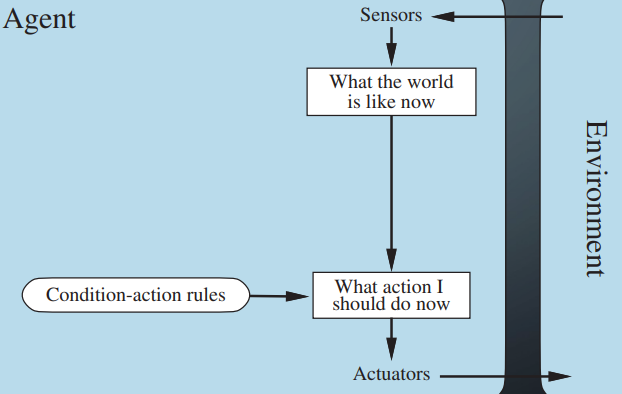
\includegraphics[width=0.25\textwidth]{./img/Agenti/SimpleReflexAgents.png}
              \caption{Schema di un agente}
              \label{fig:simpleReflex}
          \end{figure}
    \item \textbf{Model-based reflex agents}: mantiene uno stato interno che permette 
          di modellare lo storico delle percezioni che riceve dall'ambiente e sceglie
          l'azione in base al suo stato interno. Per aggiornare lo stato interno 
          in base al cambiamento dell'ambiente ci servono 2 diverse conoscenze, ciascuna
          modellata da due diversi modelli:
          \begin{itemize}
            \item \textbf{transition model}: informazioni in merito
            al cambiamento del mondo nel tempo, queste vengono raccolte dall'analisi
            dell'effetto delle azioni dell'agente e dall'evoluzione dell'ambiente 
            indipendentemente dalle azioni dell'agente.
            \item \textbf{sensor model}: informazioni in merito
            a come si riflette il cambiamento del mondo nelle percezioni dell'agente
          \end{itemize} 
          L'insieme del transition e del sensor model permette all'agente di tenere
          traccia del mondo.
          \begin{figure}[!h]
              \centering
              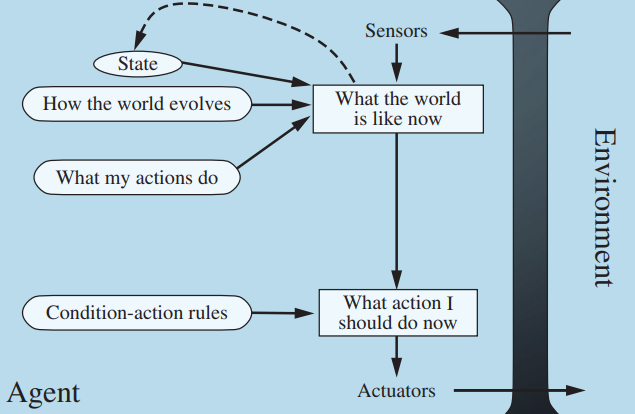
\includegraphics[width=0.25\textwidth]{./img/Agenti/ModelBasedReflexAgent.png}
              \caption{Schema di un agente}
              \label{fig:ModelReflex}
          \end{figure}
    \item \textbf{Goal-based agents}: l'agente deve sapere quali sono le
          situazioni desiderate e quali azioni devono essere svolte per raggiungere
          tali situazioni. Ha sempre una rappresentazione del mondo derivante dal 
          Model-based reflex agents, con la differenza che le decisioni prese sulla 
          rappresentazione del mondo sono dipendenti dal Goal dell'agente.
          Risultano più flessibili rispetto ai Model-based reflex agent, dato che 
          possono cambiare il comportamento solo cambiando il goal.
          \begin{figure}[!h]
              \centering
              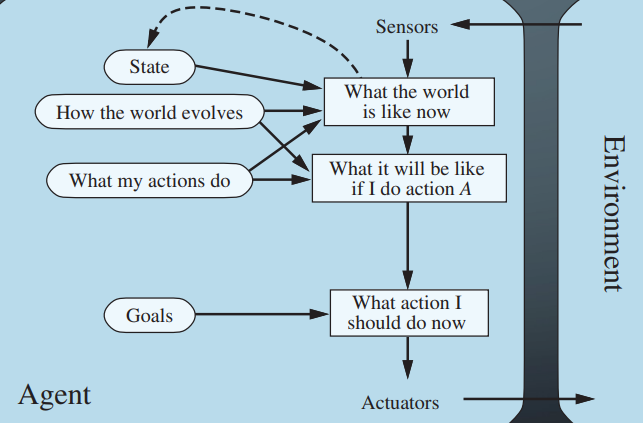
\includegraphics[width=0.25\textwidth]{./img/Agenti/GlobalBasedAgent.png}
              \caption{Schema di un agente}
              \label{fig:GoalBased}
          \end{figure}
    \item \textbf{Utility-based agents}: in questo caso uno stesso obiettivo può
          essere raggiunto in modi diversi. Viene definita una funzione di utilità che
          che descrive il grado di soddisfazione dell'agente in base alla situazione
          in cui si trova. Ho bisogno
          di una funzione utilità che mi rappresenti il mondo in modo da guidare
          le scelte dell'agente in base alla rappresentazione e i suoi obiettivi.
          \begin{figure}[!h]
              \centering
              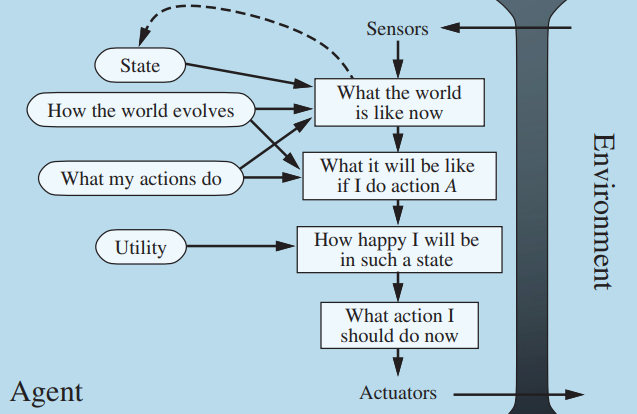
\includegraphics[width=0.25\textwidth]{./img/Agenti/UtilityBasedAgent.png}
              \caption{Schema di un agente}
              \label{fig:UtilityBased}
          \end{figure}
\end{itemize}

La prima classe di questa classificazione corrisponde alla classe degli agenti
tropistic, la seconda classe corrisponde alla classe degli agenti hysteretic. Le
altre due classi sono invece una specializzazione della classe knowledge-based.

Esistono altre classificazioni di agenti in base alle loro caratteristiche
fondamentali o in base alle capacità, un esempio sono gli agente di interfaccia.
Oltre a queste classificazioni possiamo distinguere agenti ibridi e sistemi
eterogenei.
\begin{esempio}[Esempio di agenti reattivi (Boids)]
    Agenti che simulano il comportamento di stormi di uccelli. Il comportamento
    è ottenuto mischiando i seguenti comportamenti:
    \begin{itemize}
        \item \textbf{Separazione}: ciascun Boids ha un raggio e riesce a percepire
              altri boids o ostacoli all'interno del raggio. Si ha un contributo
              nell'accelerazione verso la direzione opposta per evitare
              l'affollamento tra gli altri.
        \item \textbf{Coesione}: il Boids si muove verso la posizione centrale
              tra i vicini.
        \item \textbf{Allineamento}: orientamento spaziale deve conformarsi con
              i Boids adiacenti.
    \end{itemize}
    I comportamenti vengono uniti mediante una combinazione lineare e dei pesi.
\end{esempio}
Gli agenti reattivi non hanno obiettivi, si possono anche chiamare behaviour-based.
L'agente però è semplice computazionalmente, se voglio più complessità come per
esempio degli obiettivi allora devo complicare il modello.
\begin{esempio}[Esempio di agenti mentalistici (3APL)]
    L'agente prevede la specifica di un comportamento cognitivo mediante un
    linguaggio logico. Questo è caratterizzato da:
    \begin{itemize}
        \item Azioni base: singole azioni
        \item Belief base: insieme di fatti noti sul mondo, possono essere anche
              regole (base di conoscenza del mondo)
        \item Regole pratiche di ragionamento: insiemi di piani parzialmente istanziati,
              insieme di passi generiche che mi portano all'obiettivo
        \item Obiettivi
    \end{itemize}
    Esempio robot:
    \begin{itemize}
        \item Belief base: descrizione del mondo in PL.
        \item Capability: descrizione delle capacità (azione base) che può fare
              l'agente con la specifica di come deve essere aggiornata la base
              di conoscenza.
        \item Goal: obiettivo è la testa di una regola di un piano
        \item Rule base: insieme di piani, insieme di regole da mettere in pratica
              per portare a termine il piano e quindi l'obiettivo.
    \end{itemize}

    Hanno diversi problemi:
    \begin{itemize}
        \item Devono avere la rappresentazione completa del mondo (ambiente può
              essere molto grande)
        \item La percezione perde di significativo
        \item Come unisco reazione e deliberazione
    \end{itemize}
\end{esempio}
\begin{esempio} [Jade platform]
    Piattaforme SW per lo sviluppo di agenti, forniscono solo uno "standard SW"
    per eseguire comportamenti. L'agente viene eseguito dall'ambiente che sveglia
    chi deve eseguire e non vengono eseguiti su Thread. Quindi
\end{esempio}

Gli agenti come mostra Jade possono essere a oggetti, ma ci possono essere differenze:
\begin{itemize}
    \item \textbf{Autonomia}: un agente può fornire servizi ma non devono
          rispondere a tutte le richieste.
    \item \textbf{Pro-attività}: un agente deve avere almeno un thread per il
          suo controllo, gli oggetti in Jade non vengono eseguiti su thread.
    \item \textbf{Abilità sociale}: per gli oggetti non si hanno comunicazione
          sociale perché è limitata alla sua interfaccia che non è abbastanza
          espressiva rispetto ad un modello sociale di comunicazione.
\end{itemize}
Gli agenti possono essere visti come una specializzazione degli oggetti comuni.
\subsection{Agenti ibridi}
Gli agenti ibridi sono una tipologia di agenti intelligenti aventi una struttura
composta da strati. Ogni strato implementa un comportamento specifico.
L'architettura può essere espressa come specifiche comportamentali a layer che
può essere:
\begin{itemize}
    \item Orizzontale: una singola percezione può portare all'attivazione di due
          comportamenti paralleli.
    \item Verticale: si ha una gerarchia con priorità sui comportamenti più
          importanti.
\end{itemize}
% ! Immagine di un agente ibrido
\subsection{Sistema eterogeneo}
Un sistema complesso può integrare quindi diverse tipologie di agenti
(sistema eterogeneo), diventa fondamentale la loro interazione, specificando dei
meccanismi di interazione (ex: robot spaziali).

L'autonomia degli agenti può avere diverse declinazioni:
\begin{itemize}
    \item Capacità di un agente di decidere le proprie azioni in base allo stimolo
          esterno.
    \item Abilità di decidere in base alla sua conoscenza.
\end{itemize}
\subsection{Learning agent}
I learning agent sono agenti che integrano un processo di apprendimento. Nello
specifico contengono:
\begin{itemize}
    \item \textbf{Learning element}: l'agente apprende e modifica il suo comportamento
          in base alle percezioni. Contiene l'algoritmo di apprendimento.
    \item \textbf{Performance element}: l'agente sceglie le azioni in base alle
          percezioni. Contiene il modello appreso.
\end{itemize}
% ! Immagine di un learning agent

Se l'agente contiene un learning element allora può apprendere durante la sua vita,
altrimenti l'apprendimento può essere fatto a priori e quindi l'agente è solo il
risultato del processo. Nel caso in cui il learning element non sia presente
l'agente non è definito come learning agent.

Spesso questi agenti vengono allenati utilizzando tecniche di reinforcement
learning, ovvero gli agenti compiono delle azioni e come risposta all'azione
ottengono un punteggio che li premia o penalizza. In questo modo l'agente esplora
l'effetto delle azioni nell'immediato o nel lungo termine.